% Introdução

\documentclass[Tese.tex]{subfiles}

\begin{document}
	
\chapter{Mecânica do contínuo}\label{ch:mecanica-dos-solidos}

\textcolor{red}{sugiro alterar o título dessa seção para algo como elasticidade não linear, ou então separar o que é puramente mecânica do contínuo da parte que é aplicada a sólidos elásticos e abrir um outro capítulo para elasticidade}

A mecânica do contínuo é o ramo da mecânica que ocupa-se em descrever o comportamento de materiais, tais como sólidos ou fluidos, sem considerar sua estrutura molecular ou granular, ou seja, tratando-os como meios contínuos. Ela se baseia na suposição de que, na escala de interesse, esses materiais podem ser considerados como uma entidade contínua e homogênea, em oposição aos modelos que descrevem o comportamento dos materiais em nível molecular.

Usualmente, a mecânica do contínuo possui duas formas principais de descrição: a Lagrangiana, ou material, onde toma-se como referência uma configuração de equilíbrio do corpo (a configuração inicial do corpo no caso da descrição Lagrangiana total), e a Euleriana, ou espacial, onde toma-se como referência a configuração deformada atual do corpo. Neste trabalho, opta-se por utilizar a descrição Lagrangiana. Maiores detalhes sobre os temas abordados aqui podem ser encontrados em \citeonline{ogden1997non,bonet1997nonlinear} e \citeonline{CodaLivro}.

\textcolor{red}{Faltou dizer porque (justificar) você está optando pela descrição Lagrangiana}

\section{Cinemática dos corpos deformáveis}\label{sec:cinematica}

Seja um corpo com configuração inicial ou indeformada $\domVoli$, e configuração atual $\domVol$. Define-se a {função mudança de configuração} $\funcao$ como sendo uma aplicação vetorial que mapeia as posições atuais (denotadas por $\y$) a partir das iniciais (denotadas por $\x$), conforme ilustra a \autoref{fig:cinematica}. Denota-se por $\F$ o gradiente da função mudança de configuração, isto é:
\begin{equation}\label{eq:A}
\F = \gradientei\cdot\funcao.
\end{equation}
onde $\gradientei$ denota o gradiente com relação à configuração inicial.

\begin{figure}[h]
	\centering
	\caption{Mudanças de configuração de um corpo deformável}
	\label{fig:cinematica}
	{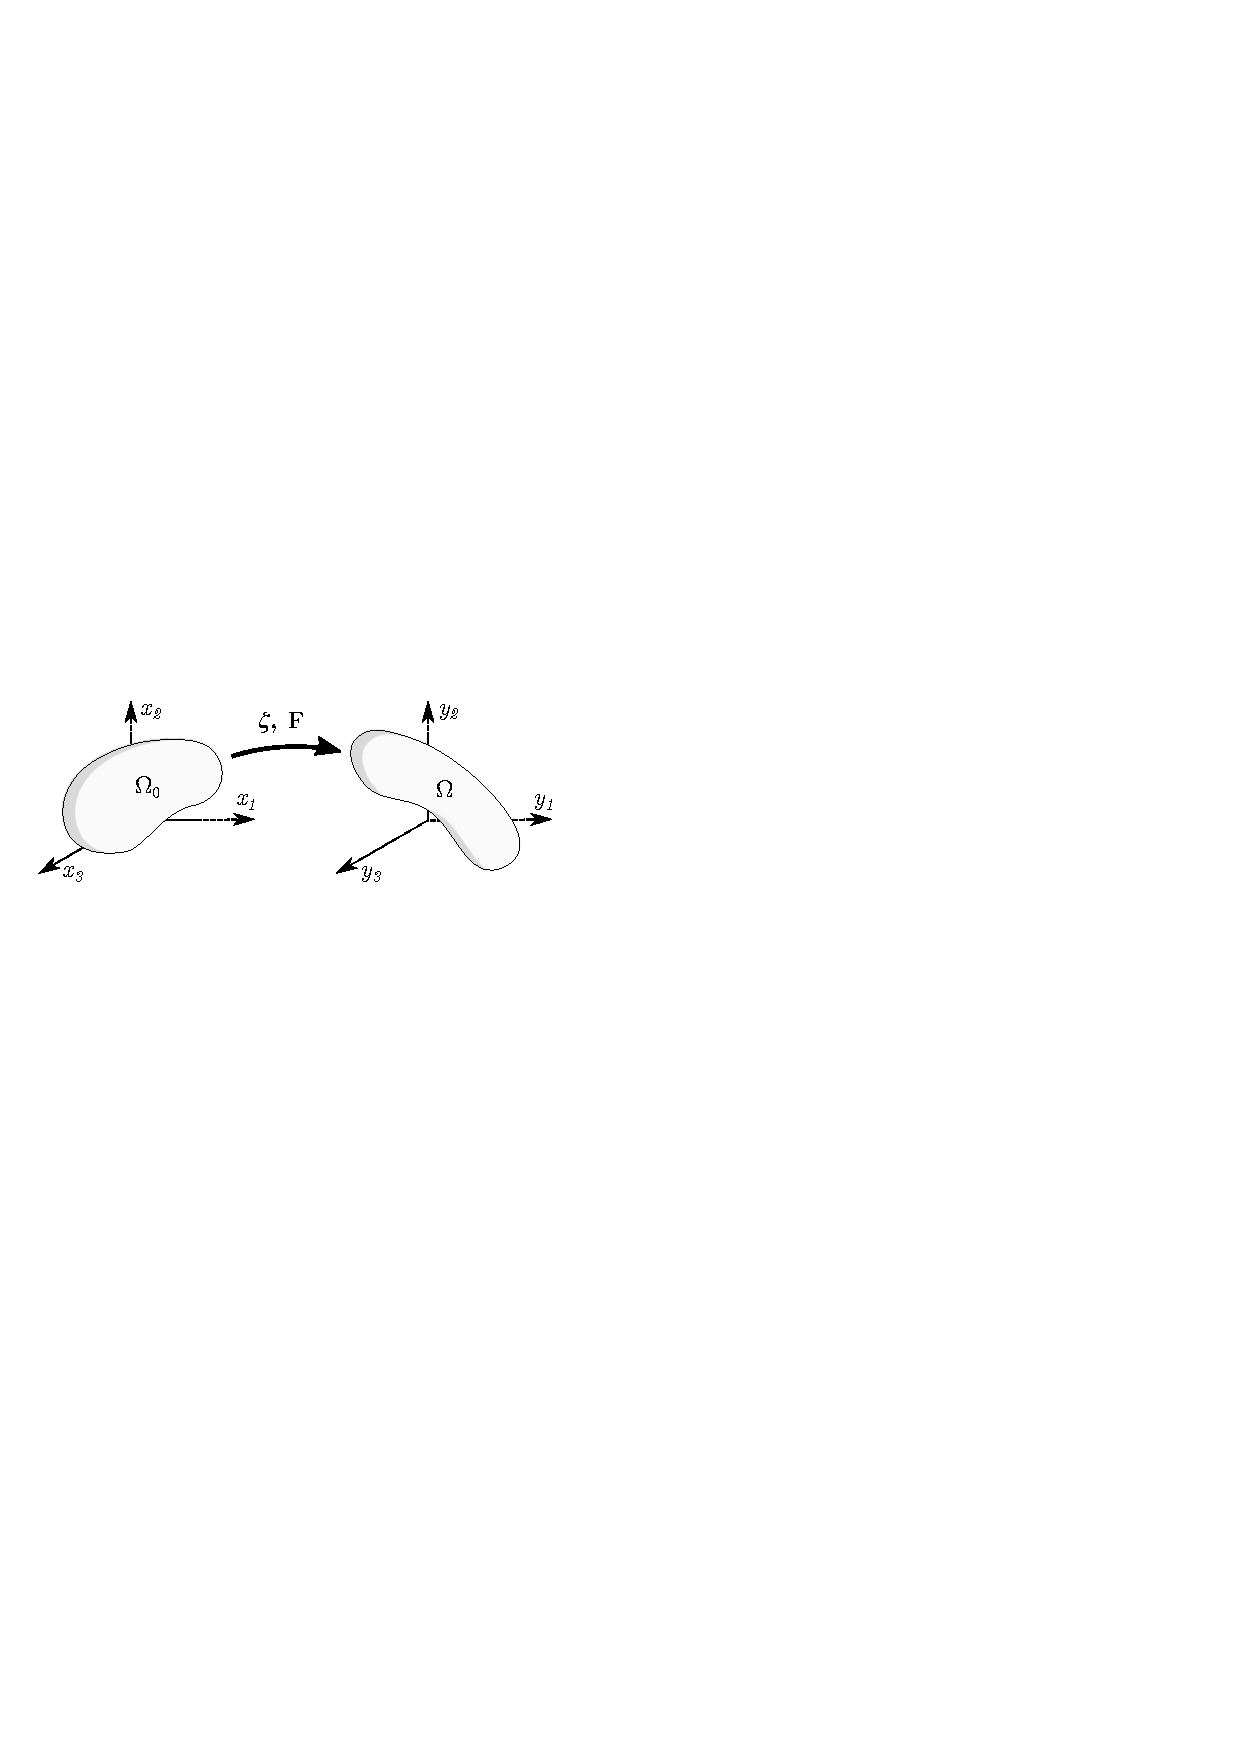
\includegraphics[scale=1.0]{Figuras/kinematics0.pdf}}	
	\caption*{\textbf{Fonte:} \citeonline{Pericles2019}}
\end{figure}

\subsection{Medidas de deformação}

Uma medida de deformação é uma grandeza adimensional que permite mensurar pontualmente a mudança de forma ocorrida entre as configurações inicial e atual. Neste trabalho, as principais medidas de deformação utilizadas são o alongamento à direita de Cauchy-Green $\C$ e o tensor de deformação de Green-Lagrange $\E$, definidos respectivamente por:
\begin{align}
&\C=\F^T\F \label{eq:alongamentocauchy},\\[0.1cm]
&\E = \dfrac{1}{2}(\C-\I). \label{eq:E}
\end{align}
Uma vez que $\F$ é definido na configuração inicial, segue que as medidas de deformação apresentadas são Lagrangianas. Além disso, é possível demonstrar que elas são objetivas, isto é, independem de movimentos de corpo rígido. Na ausência de deformações, temos $\C=\F=\I$ e $\E=\mathbf{0}$. Outra característica conveniente do tensor de Green-Lagrange é que, para pequenas deformações, ela se aproxima à deformação linear de engenharia ($\defLinear$), recuperando os resultados da mecânica linear.

A taxa da deformação de Green-Lagrange pode ser calculada a partir da \cref{eq:E} como
\begin{equation}\label{eq:dotE}
\dotE = \dfrac{1}{2}\left(\dotF^T\F+\F^T\dotF\right),
\end{equation}
onde 
\begin{equation}
\dotF = \gradientei\cdot\dotfuncao.
\end{equation}

Outra grandeza de particular utilidade neste trabalho é o gradiente da velocidade da mudança de configuração, definido por $\L = \gradiente\cdot\dotfuncao$, onde $\gradiente$ denota o gradiente com relação à configuração atual e o ponto sobrescrito $\dot{(\;\,)}$ indica derivada no tempo. Apesar de ser uma grandeza Euleriana, ele pode ser escrito em termos de $\F$ pela seguinte relação:
\begin{equation}\label{eq:gradiente-velocidade}
\L = \dfrac{\partial\dotfuncao}{\partial\y}=\dfrac{\partial\dotfuncao}{\partial\x}\dfrac{\partial\x}{\partial\y} = \dotF\F^{-1}.
\end{equation}
Pode-se ainda decompor $\mathbf{L}$ em suas parcelas simétrica e antissimétrica, isto é:
\begin{align}
\L &= \D+\W, \text{\quad onde} \\
\D &= \Sim(\L)=\dfrac{1}{2}(\L+\L^T) \text{,\; e} \label{eq:taxa-deformacao} \\
\W &= \Ant(\L)=\dfrac{1}{2}(\L-\L^T) \label{eq:vorticidade}  \text{.\quad\,\;}
\end{align}
O tensor $\D$, também representado por $\dotDefLinear$, é denominado taxa de deformação, enquanto $\W$ é denominado tensor taxa de rotação, ou vorticidade, ambos medidas Eulerianas. Aplicando \eqref{eq:taxa-deformacao} em \eqref{eq:dotE}, chega-se à seguinte relação entre $\D$ e a taxa de deformação de Green-Lagrange:
\begin{equation}
\dotE = \F^{T}\D\F \text{.} \label{eq:taxa-green-2}
\end{equation}

\subsection{Fórmulas da mudança de volume e área}\label{sec:mudancavol}

Seja um elemento infinitesimal com volumes na configuração inicial e na configuração atual denotados por $d\voli$ e $d\vol$, respectivamente. Pode se estabelecer a seguinte relação entre a variação de volume e o gradiente da função mudança de configuração:
\begin{equation}\label{eq:mudanca-volume}
\J = \det\F = \dfrac{d\vol_{\;}}{d\voli},
\end{equation}
onde $\J$ é chamado de determinante Jacobiano, sendo uma medida de deformação volumétrica. A \cref{eq:mudanca-volume}, denominada fórmula da mudança de volume, estabelece ainda uma importante condição: como os volumes são sempre grandezas positivas, segue também que $\J=\det\F$ deve sempre ser positivo maior que zero, caso contrário há uma inconsistência física no modelo, caracterizada pela destruição ou inversão da matéria.

Agora seja uma área infinitesimal denotada por $d\coni$ na configuração inicial e $d\con$ na configuração atual, e sejam $\normali$ e $\normal$, respectivamente, os vetores unitários ortogonais à essas áreas. É possível estabelecer a seguinte relação:
\begin{equation}\label{eq:mudanca-area}
\F\cdot\normal\, d\con = J\normali\, d\coni,
\end{equation}
denominada fórmula de Nanson, ou fórmula da mudança de área. 

As \cref{eq:mudanca-volume,eq:mudanca-area} são utilizadas em diversas passagens deste texto para relacionar equações Lagrangianas e Eulerianas. As demonstrações de ambas podem ser encontradas, por exemplo, em \citeonline{CodaLivro}.

\subsection{Princípio da conservação da massa}\label{sec:conservacao-massa}

Outra propriedade que deve ser observada no equacionamento dos problemas mecânicos, e que auxilia a conversão de equações Lagrangianas em Eulerianas e vice-versa, é o princípio da conservação da massa. Esse princípio estabelece que os volumes de um corpo contínuo nas suas configurações inicial ($\voli$) e atual ($\vol$) deverá ter a mesma massa. Assim, denotando por $d\Mass$ a massa de um volume infinitesimal, e aplicando a fórmula da mudança de volume, temos:
\begin{equation}\label{eq:conservacao-massa}
\massi = \dfrac{d\Mass}{d\voli} = J\dfrac{d\Mass}{d\vol} = J\mass,
\end{equation}
onde $\massi$ e $\mass$ são as densidades de massa nas configurações inicial e final, respectivamente. Pode-se ainda expressar a \cref{eq:conservacao-massa} na forma
\begin{equation}\label{eq:conservacao-massa2}
\massi\,d\voli = \mass\,d\vol.
\end{equation}
Logo, apesar de $\mass$ e $d\vol$ serem variáveis no tempo, o produto $\rho\,d\vol$ é constante. Como consequência, sendo $f$ uma função qualquer dependente do tempo, a seguinte propriedade pode ser garantida:
\begin{equation}\label{eq:conserv5}
\dfrac{d}{dt}\int_{\domVol}\mass f\,d\vol = \dfrac{d}{dt}\int_{\domVoli}\massi f\,d\voli = \int_{\domVoli}\massi \dot{f}\,d\voli = \int_{\domVol}\mass \dot{f}\,d\vol,
\end{equation}
onde $\dot{f}$ é a derivada material de $f$ no tempo.

\section{Equilíbrio}\label{sec:equilibrio}

Neste trabalho, as equações de equilíbrio são obtidas por meio da abordagem energética, partindo-se do princípio da energia total estacionária. Escreve-se o funcional da energia mecânica total do sistema como	
\begin{equation}
\Energiamec = \Energiadef + \Energiacin - \Energiaext , \label{eq:energy}
\end{equation}	
\noindent onde $\Energiadef$ é a energia de deformação, $\Energiacin$ é a energia cinética e $\Energiaext$ é a energia potencial das forças externas. O princípio da conservação da energia implica que a primeira variação do funcional deve ser nula, isto é,	
\begin{equation}\label{eq:conservacao-energia}
\delta\Energiamec = \delta\Energiadef + \delta\Energiacin - \delta\Energiaext = 0 .
\end{equation}

\textcolor{red}{Até aqui é só conservação da energia. Estacionariedade da Energia é quando, partindo dessa equação, você estabelece que o ponto de equilibrio é um ponto estacionário, ou seja, é aquele em que as primeiras derivadas do funcional em relação às incógnitas que definem o funcional não nulas... Acrescente essa equação.} 

Uma vez definidas as parcelas de energia, a \cref{eq:conservacao-energia} fornece as condições necessárias para o equilíbrio do sistema. Além disso, a segunda variação de $\Energiamec$ pode fornecer informações à respeito da natureza do equilíbrio: caso positivo, esse é estável; caso negativo, é instável; caso nulo, é indiferente.

\subsection{Energia de deformação}\label[subsec]{subsec:energiadef}

A energia de deformação está relacionada ao trabalho devido que pode ser realizado pelas forças internas, podendo ser escrita pela integral
\begin{equation}\label{eq:pidef}
\Energiadef = \int_{\domVoli}\helmholtz\,d\voli,
\end{equation}
onde $\helmholtz$ é a energia específica de deformação, ou energia livre de Helmholtz, definida pelo modelo constitutivo do material. Uma vez que a formulação descrita é totalmente Lagrangiana, a integral \eqref{eq:pidef} é calculada no volume inicial, e, portanto, $\helmholtz$ deve ser definida em termos da configuração inicial. A variação da energia de deformação pode ser escrita como
\begin{equation}\label{eq:dpidef}
\delta\Energiadef = \int_{\domVoli}\delta\helmholtz\,d\voli = \int_{\domVoli}\dfrac{\partial\helmholtz}{\partial\E}:\delta\E\,d\voli = \int_{\domVoli}\S:\delta\E\,d\voli = \dfrac{1}{2}\int_{\domVoli}\S:\delta\C\,d\voli,
\end{equation}
onde 
\begin{equation}\label{eq:S}
\S=\dfrac{\partial \helmholtz}{\partial\E}
\end{equation}
é uma medida de tensão denominada tensor de Piola-Kirchhoff de segunda espécie. Embora $\S$ não apresente significado físico explícito, é possível, a partir de manipulações algébricas \cite{CodaLivro}, relaciona-lo ao tensor das tensões de Cauchy, $\cauchy$, pela expressão:
\begin{equation}\label{eq:cauchy}
\cauchy = \dfrac{1}{\J}\F\S\F^T,
\end{equation}	
de onde pode-se concluir também que $\S$ é simétrico. A relação entre $\S$ e $\E$ estabelecida pela \cref{eq:dpidef} é denominada conjugação energética, isto é, diz-se que $\S$ é conjugado energético de $\E$. %, uma vez que:
%	\begin{equation}
%	\S^T = \dfrac{1}{J}(\F^{-1}\s\F^{-T})^T = \dfrac{1}{J}\F^{-1}\s^T\F^{-T} = \dfrac{1}{J}\F^{-1}\s\F^{-T} = \S
%	\end{equation}

%	A partir da \cref{eq:dpsi} escreve-se, enfim, a variação da energia de deformação:
%	\begin{equation}\label{eq:dpidef}
%	\delta\helmholtz = \int_{\domVoli}\S:\delta\E\,d\voli = \dfrac{1}{2}\int_{\domVoli}\S:\delta\C\,d\voli.
%	\end{equation}


%Além disso, a \cref{eq:dpidef} pode ser escrita em termos de quaisquer pares conjugados de medidas de tensão e deformação. Uma forma alternativa comumente utilizada é
%\begin{equation}\label{eq:dpidef2}
%\delta\Energiadef = \int_{\domVoli}\dfrac{\partial\helmholtz}{\partial\F}:\delta\F\,d\voli = \int_{\domVoli}\P^T:\delta\F\,d\voli,
%\end{equation}
%onde $\P=\partial\helmholtz/\partial\F$ é denominado tensor de Piola-Kirchhoff de primeira espécie, conjugado energético do gradiente da função mudança de configuração. Esse pode ser relacionado aos demais tensores por
%\begin{equation}
%\P = \J\F^{-1}\cauchy = \S\F^T,
%\end{equation}
%no entanto, sua simetria não pode ser garantida.

\subsection{Energia cinética}

A energia cinética está relacionada aos movimentos do corpo, sendo escrita como:
\begin{equation}\label{eq:picin}
\Energiacin = \dfrac{1}{2}\int_{\domVol}\mass \doty\cdot\doty\,d\vol = \dfrac{1}{2}\int_{\domVoli}\massi \doty\cdot\doty\,d\voli, \\
\end{equation}
onde $\mass$ e $\massi$ são a densidade de massa do material na configuração atual e inicial, respectivamente, e $\y$ é o campo de posições atuais. A passagem da primeira para a segunda forma na \cref{eq:picin} é feita por meio do princípio da conservação da massa. 

A variação da energia cinética pode ser calculada com auxílio da derivada temporal, isto é:
\begin{equation}\label{eq:dpicin}
\delta\Energiacin = \dfrac{1}{2}\int_{\domVoli}\massi \dfrac{d}{dt}(\doty\cdot\doty)\delta t\,d\vol = \int_{\domVoli}\massi \ddoty\cdot\doty\delta t\,d\voli = \int_{\domVoli}\massi \ddoty\cdot\delta \y\,d\voli, \\
\end{equation}
onde na última passagem considerou-se que $\doty\delta t = \delta\y$.

\subsection{Energia potencial das forças externas}\label{subsec:externas}

Assumindo que o corpo esteja sujeito a forças de superfície e de volume, denotadas por $\forcaContorno$ e $\forcaVolume$, respectivamente, podemos escrever a energia potencial das forças externas como
\begin{equation}\label{eq:piext}
\Energiaext = \int_{\domConi}\forcaContorno\cdot \y\,d\coni + \int_{\domVoli}\forcaVolume\cdot \y\,d\voli.
\end{equation}
Embora tenha sido omitida a notação $\notacaoInicial$, assume-se que $\forcaContorno$ e $\forcaVolume$ são definidas na configuração inicial. Considerando ainda que essas sejam conservativas, isto é, independentes da mudança de posição, temos:
\begin{equation}\label{eq:dpiext}
\delta\Energiaext = \int_{\domConi}\forcaContorno\cdot \delta\y\,d\coni + \int_{\domVoli}\forcaVolume\cdot \delta\y\,d\voli.
\end{equation}

%\subsection{Forma global e local da equação de equilíbrio Lagrangiana}
%
%Aplicando as \cref{eq:dpidef,eq:dpicin,eq:dpiext} na \cref{eq:conservacao-energia}, obtemos a chamada equação global de equilíbrio em forma variacional:	
%\begin{equation}\label{eq:equilibrio-global}
%\delta\Pi = \int_{\domVoli}\S:\delta\E\,d\voli + \int_{\domVoli}\massi \ddoty\cdot\delta \y\,d\voli - \int_{\domConi}\forcaContorno\cdot \delta\y\,d\coni - \int_{\domVoli}\forcaVolume\cdot \delta\y\,d\voli = 0.
%\end{equation}
%
%Conforme visto na \cref{eq:dpidef2}, $\S:\delta\E$ pode ser substituído por $\P^T:\delta\F = \P^T:(\gradientei\cdot\delta\y)$. Pela regra do produto, $\gradientei\cdot(\P^T\cdot\delta\y) = \P^T:(\gradientei\cdot\delta\y) + (\gradientei\cdot\P^T)\cdot\delta\y$. Logo:
%\begin{equation}\label{eq:temp1}
%\int_{\domVoli}\S:\delta\E\,d\voli = \int_{\domVoli}\gradientei\cdot(\P^T\cdot\delta\y)\,d\voli - \int_{\domVoli} (\gradientei\cdot\P^T)\cdot\delta\y\,d\voli.
%\end{equation}
%Ainda, pelo teorema da divergência, temos:
%\begin{equation}\label{eq:temp2}
%\int_{\domVoli}\gradientei\cdot(\P^T\cdot\delta\y)\,d\voli = \int_{\domConi} (\P^T\cdot\delta\y)\cdot\normali\,d\coni = \int_{\domConi} (\P^T\cdot\normali)\cdot\delta\y\,d\coni.
%\end{equation}
%Aplicando as \cref{eq:temp1,eq:temp2} na \cref{eq:equilibrio-global}, temos, portanto:
%\begin{equation}
%\delta\Pi = \int_{\domConi} (\P^T\cdot\normali-\forcaContorno)\cdot\delta\y\,d\coni + \int_{\domVoli}(\massi \ddoty-\gradientei\cdot\P^T-\forcaVolume)\cdot\delta \y\,d\voli = 0.
%\end{equation}
%Pela arbitrariedade de $\delta\y$, temos, no contorno do corpo, a seguinte equação relacionando o vetor de forças distribuídas na superfície com o tensor de Piola-Kirchhoff de segunda espécie:
%\begin{equation}
%\P^T\cdot\normali = \forcaContorno,
%\end{equation}
%e, no domínio do corpo, temos a chamada equação de equilíbrio Lagrangiana local:
%\begin{equation}
%\massi \ddoty-\gradientei\cdot\P^T-\forcaVolume = \mathbf{0}.
%\end{equation}

\textcolor{red}{Daqui em diante você está resolvendo especificamente a mecânica dos sólidos}

\section{Modelos constitutivos hiperelásticos}\label{sec:hiper}

Diz-se que um modelo constitutivo é elástico quando é definido apenas em função do estado de deformação atual, e independe de fatores como histórico e taxa de deformação. Quando, além disso, esse deriva de uma expressão explícita para $\helmholtz$, diz-se que o modelo é hiperelástico. Para garantir que esse seja independente da escolha de eixos coordenados, escreve-se $\helmholtz$ em função dos invariantes de $\C$, definidos como
\begin{align}
& \invar = \tr(\C) ,\\
& \invarr = \dfrac{1}{2}\left[\tr(\C)^2-\tr(\C^2)\right] \text{,\; e}\\
& \invarrr = \det(\C),
\end{align}
ou dos invariantes de $\E$, definidos de forma análoga.

\subsection{Modelo de Saint Venant-Kirchhoff}

O modelo de Saint Venant-Kirchhoff é considerado o caso mais simples de lei hiperelástica, relacionando linearmente o tensor de Piola-Kirchhoff de segunda espécie com a deformação de Green-Lagrange. Neste caso, define-se a energia específica de deformação em termos dos invariantes de $\E$, pela expressão:
\begin{equation}\label{eq:ue-SVK}
\helmholtz = \dfrac{1}{2}(\lame-\G)\invar^2 + \G \invarr = \G \,\tr(\E^2)+\dfrac{1}{2}\lame\,\tr(\E)^2,
\end{equation}
onde $\lame$ e $\G$ são o parâmetro de Lamé e o módulo de elasticidade transversal do material, respectivamente, que podem ser relacionadas com o módulo de elasticidade ($\young$) e coeficiente de Poisson ($\poisson$) pelas expressões:
\begin{equation}
\lame = \dfrac{\poisson \young}{(1+\poisson)(1-2\poisson)}
\qquad\text{e}\qquad
\G = \dfrac{\young}{2(1+\poisson)}. \label{eq:lame}
\end{equation}
Da \cref{eq:ue-SVK}, podemos calcular a tensão de Piola-Kirchhoff de segunda espécie como:
\begin{equation}
\S = \dfrac{\partial \helmholtz}{\partial \E} = \lame\,\tr(\E)\I + 2\G\E.
\end{equation}
Além disso, define-se o operador tangente consistente como:
\begin{equation}\label{eq:C-SVK}
\CC = \dfrac{d \S}{d \E} = 2\G\II + \lame\I\otimes\I.
\end{equation}
\textcolor{red}{O que é $\II$? VocÊ tem certeza sobre essa equação? Dê uma conferida para garantir, é que eu já acabei tendo problemas com essa notação para o tensor constitutivo uma vez... Peguei de um lugar que estava errado.}
Observa-se que, neste modelo, $\CC$ é constante, o que permite que a lei de Saint Venant-Kirchhoff seja escrita na seguinte forma simplificada:
\begin{align}
&\helmholtz = \dfrac{1}{2}\,\E:\CC:\E,\\[0.1cm]
&\S = \CC:\E.
\end{align}

Apesar de simples, a lei de Saint Venant-Kirchhoff deve ser limitada ao caso de pequenas deformações, uma vez que essa permite a inversão do material, isto é, valores negativos de jacobiano, quando submetida à tensões compressivas excessivas.

\subsection{Modelo Neo-Hookeano}\label{subsec:neo-hoookean}

Para problemas envolvendo grandes deformações, utiliza-se neste trabalho o modelo constitutivo Neo-Hookeano definido pela seguinte energia específica de deformação:
\begin{equation}\label{eq:neoHookean2}
\helmholtz = \dfrac{\lame}{2}\left(\ln\sqrt{\invarrr}\right)^2 + \dfrac{\G}{2}\left(\tr\C - 3 - \ln\sqrt{\invarrr}\right) = \dfrac{\lame}{2}(\ln\,\J)^2 + {\G}\left(\tr\E - \ln\J\right) .
\end{equation}
Desse modelo, derivam as seguintes expressões para o tensor de Piola-Kirchhoff de segunda espécie e operador tangente consistente:
\begin{align}
&\S=\lame\ln(\J)\C^{-1} + \G(\I-\C^{-1}), \\[0.1cm]
&\CC=\lame\C^{-1}\otimes\C^{-1}+2\lame\ln(\J)\dfrac{\partial\C^{-1}}{\partial\C^{\;\;}} - 2\G\dfrac{\partial\C^{-1}}{\partial\C^{\;\;}} .
\end{align}

É possível demonstrar que, para deformações suficientemente pequenas, o modelo Neo-Hookeano se assemelha ao modelo de Saint Venant-Kirchhoff, e ambos se assemelham à lei de Hooke generalizada.

\textcolor{red}{Acho importante adicionar referências para as principais medidas e modelos apresentados aqui. Pode colocar referências gerais no início do capítulo de Mecânica do contínuo ou local. Quando estiver fazendo isso, tente usar livros voltados à mecânica do contínuo como Holzapfel, Ogden, Crisfield... ao invés do livro do Coda.}

\subsection{Estado plano de deformação e de tensão}\label{subsec:estado-plano}

As leis constitutivas apresentadas são definidas para o caso 3D, logo os tensores envolvidos devem ser aplicados em sua forma completa $3\times 3$. No entanto, em problemas bidimensionais só é possível escrever os tensores de deformação na forma $2\times 2$, sendo necessário adotar considerações sobre os demais termos. Nesse sentido, duas aproximações são comumente adotadas: estado plano de deformação (EPD) ou estado plano de tensão (EPT).

No EPD, considera-se que as componentes de deformação que atuam na terceira dimensão são nulas, isto é, $\Eind_{13}=\Eind_{23}=\Eind_{31}=\Eind_{32}=\Eind_{33}=0$, e portanto a lei constitutiva pode ser resolvida de forma direta. Já no EPT, esses termos devem ser calculados de forma que as componentes de tensão que atuam na terceira dimensão sejam nulas, isto é, $\Sind_{13}=\Sind_{23}=\Sind_{31}=\Sind_{32}=\Sind_{33}=0$, resultando em um sistema a ser resolvido para $\Eind_{13}$, $\Eind_{23}$ e $\Eind_{33}$.

Para modelos isotrópicos, as condições $\Sind_{13}=\Sind_{23}=0$ resultam automaticamente em $\Eind_{13}=\Eind_{23}=0$, restando apenas encontrar $\Eind_{33}$ tal que $\Sind_{33}=0$. No caso da lei de Saint Venant-Kirchhoff, isso é um problema linear que pode ser resolvido de forma explícita. Já no modelo Neo-Hookeano, o problema é não-linear, sendo resolvido neste trabalho pelo método de Newton-Raphson, de acordo com os seguintes passos:
\begin{enumerate}[leftmargin=\parindent,labelwidth=\parindent,labelsep=0.3cm,noitemsep]
	\item Inicialmente, assume-se $\Eind_{33}$ nulo ou igual ao seu valor do passo anterior;
	\item Calcula-se $\S$ e $\CCind$ pela lei constitutiva; \label{itm:trial-plane-stress}
	\item Soma-se a $\Eind_{33}$ o valor $\Delta\Eind_{33}=-\Sind_{33}/\CCind_{3333}$;
	\item Se $|\Delta\Eind_{33}|$ ou $|\Sind_{33}|$ for menor que uma tolerância pré-estabelecida, finaliza-se o processo iterativo. Caso contrário, retorna-se ao \autoref{itm:trial-plane-stress}.
\end{enumerate}

Esse processo, embora computacionalmente custoso, se destaca pela sua generalidade, pois pode ser aplicado a qualquer modelo constitutivo, não se limitando aos casos hiperelásticos. Em particular, os mesmos procedimentos para o EPD e o EPT podem ser reaproveitados aos modelos termo-mecânicos e inelásticos apresentados posteriormente neste trabalho.

\section{Método dos elementos finitos aplicado ao problema mecânico}\label{sec:mef}

O problema da mecânica do contínuo é resolvido numericamente neste trabalho pelo método dos elementos finitos, utilizando a abordagem baseada em posições descrita em \citeonline{CodaLivro}, que se diferencia das tradicionais por utilizar como parâmetros nodais as posições ao invés dos deslocamentos ou velocidades. Para mais detalhes sobre a formulação, a referência citada deve ser consultada.

\subsection{Discretização espacial}

Neste trabalho, utilizam-se elementos finitos com funções de forma polinomiais de ordem 1, 2 e 3, dando preferência ao último pelos bons resultados alcançados em pesquisas relacionadas, permitindo uma melhor representação de geometria curvilíneas, e garantindo respostas satisfatórias sem que haja necessidade de refinamento excessivo da malha. No caso tridimensional, os domínios são discretizados em elementos do tipo hexaédrico, denotados por HEX8, HEX27 e HEX64, e tetraédrico, denotados por TE4, TE10 e TE20. No caso bidimensional, utilizam-se elementos quadrilaterais, denotados por Q4, Q9 e Q16, e triangulares, denotados por T3, T6 e T10. Já os contornos dos domínios bidimensionais são discretizados por elementos de linha de ordem equivalente, denotados por L2, L3 e L4. Todos os elementos citados são bem estabelecidos na literatura, tendo sido dispostos em ordem crescente de grau do polinômio, com número à direita representando a quantidade de nós em cada caso.

%\begin{figure}[!htb]
%	\centering 
%	\caption{Elementos finitos triangulares em coordenadas adimensionais}
%	\label{fig:triangulares}
%	\begin{subfigure}[t]{.33\textwidth}
%		\centering
%		\caption{T3}
%		\label{fig:T3}
%		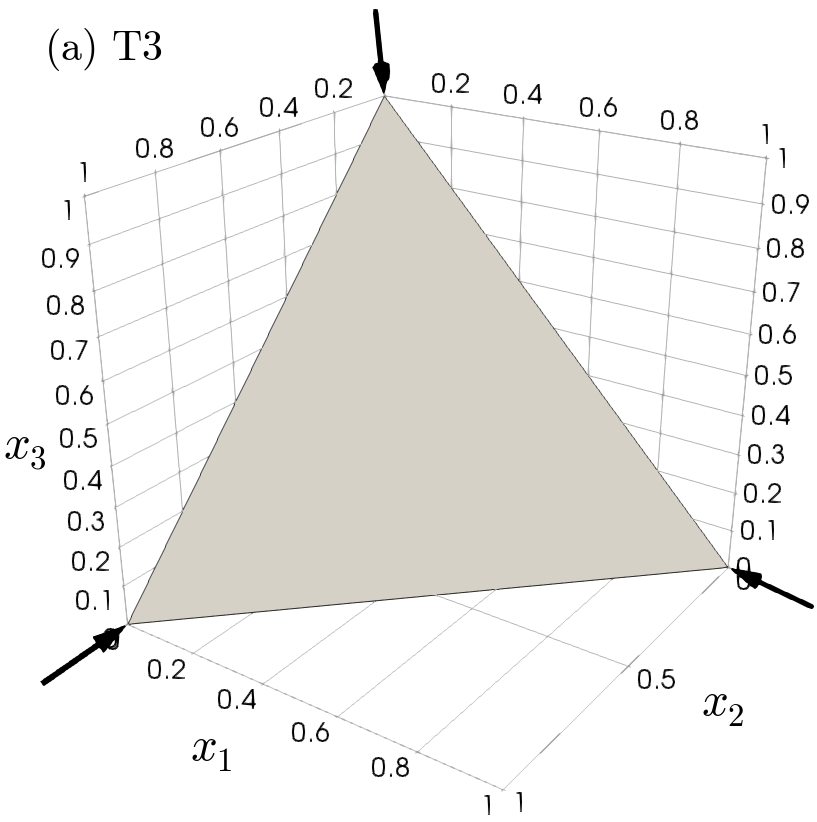
\includegraphics[scale=1]{Figuras/T3.pdf}		
%	\end{subfigure}%
%	\begin{subfigure}[t]{.33\textwidth}
%		\centering
%		\caption{T6}
%		\label{fig:T6}
%		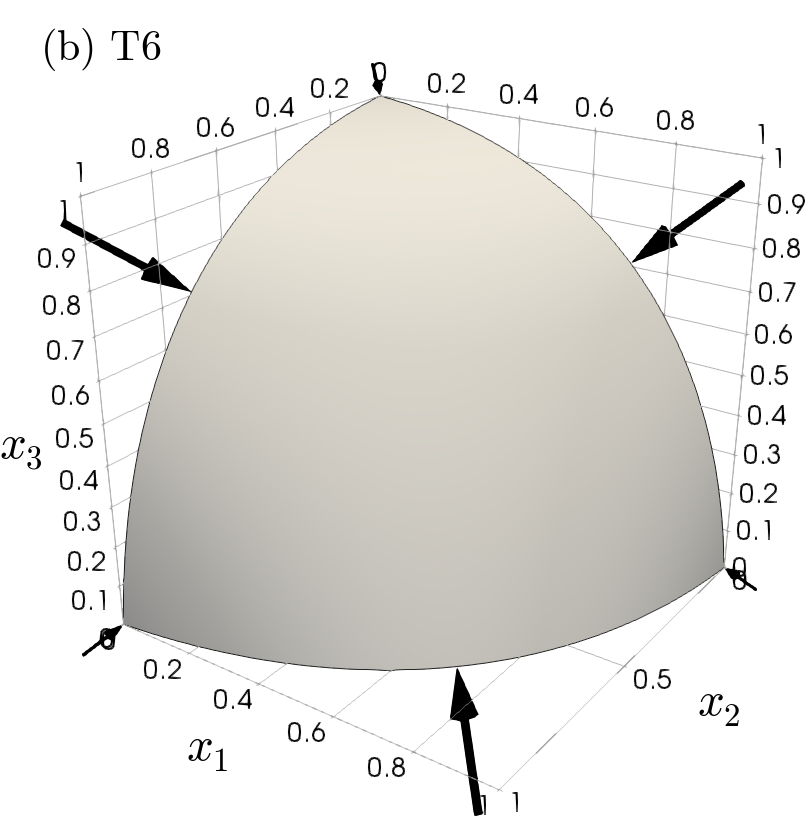
\includegraphics[scale=1]{Figuras/T6.pdf}		
%	\end{subfigure}
%	\begin{subfigure}[t]{.33\textwidth}
%		\centering
%		\caption{T10}
%		\label{fig:T10}
%		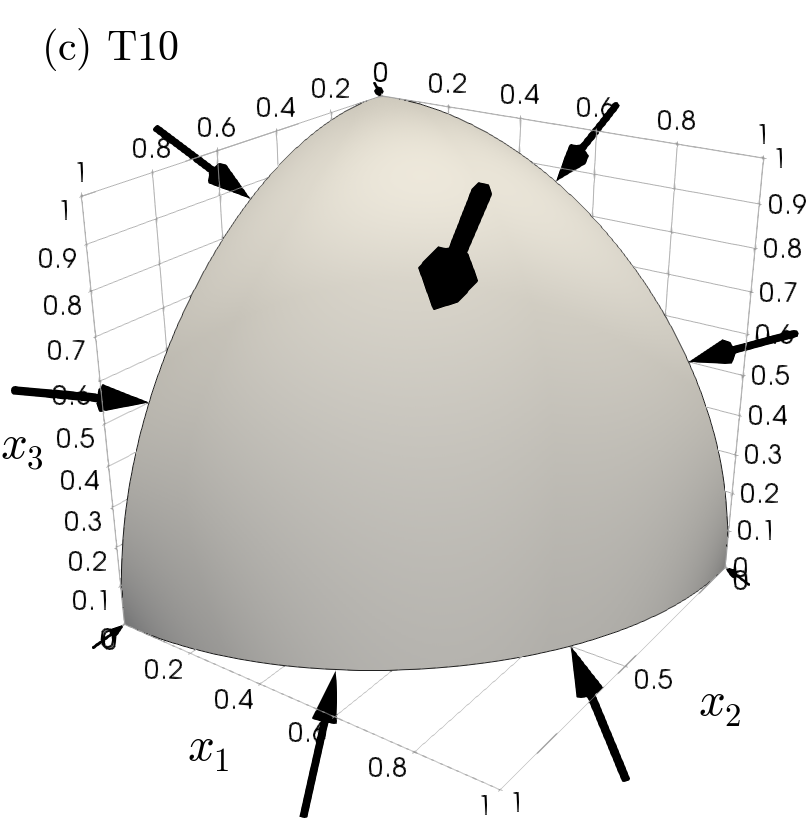
\includegraphics[scale=1]{Figuras/T10.pdf}		
%	\end{subfigure}		
%	\caption*{\textbf{Fonte:} \citeonline{Pericles2019}}
%\end{figure}

%\begin{figure}[!htb]
%	\centering 
%	\caption{Elementos finitos de linha curva em coordenadas adimensionais}
%	\label{fig:lineares}
%	%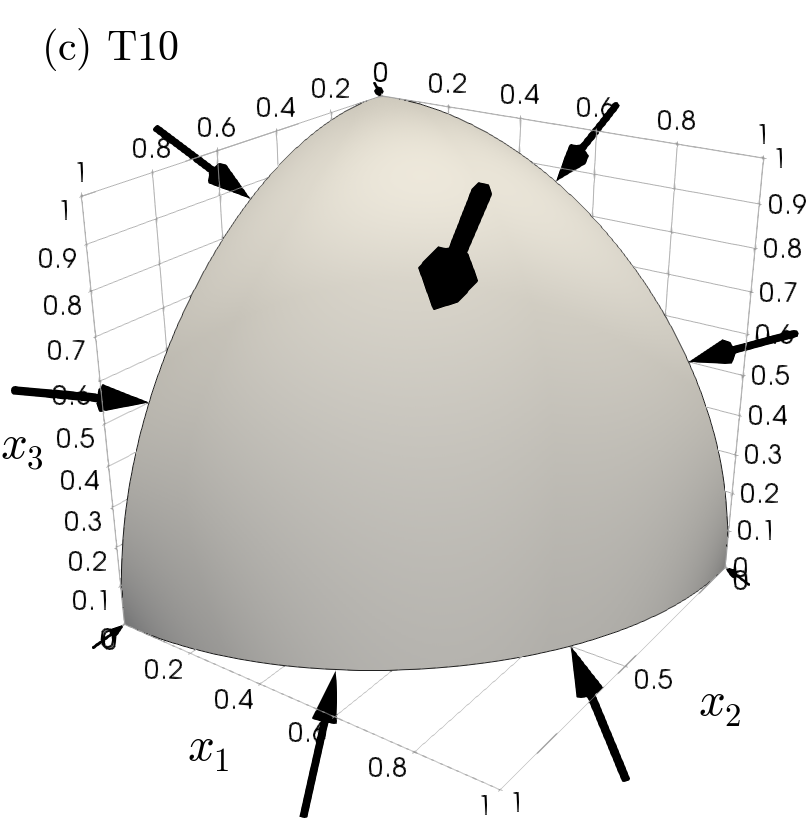
\includegraphics[scale=1.1]{Figuras/T10.pdf}
%	%\caption{Elemento finito mestre triangular com 10 nós e aproximação cúbica}
%	\begin{subfigure}[t]{.33\textwidth}
%		\centering
%		\caption{L2}
%		\label{fig:L2}
%		\includegraphics[scale=1]{Figuras/LI2.pdf}		
%	\end{subfigure}%
%	\begin{subfigure}[t]{.33\textwidth}
%		\centering
%		\caption{L3}
%		\label{fig:L3}
%		\includegraphics[scale=1]{Figuras/LI3.pdf}		
%	\end{subfigure}
%	\begin{subfigure}[t]{.33\textwidth}
%		\centering
%		\caption{L4}
%		\label{fig:L4}
%		\includegraphics[scale=1]{Figuras/LI4.pdf}		
%	\end{subfigure}		
%	\caption*{\textbf{Fonte:} \citeonline{Pericles2019}}
%\end{figure}

\textcolor{red}{Sugestão: evite usar índices sobrepostos ($\fforma\nodeind(\coords)\x\nodeind$ mudar para $\phi_{\alpha}$...), reserve isso para as potências e para indicar variável interpolada no espaço finito ex: $\F^h$. Se precisar associar índices em variável que já possui subscrito, deixe o primeiro índice entre parênteses...}

Os elementos são definidos em coordenadas adimensionais, denotadas por $\coords$, a partir das quais são mapeados os elementos nas configurações inicias e finais. Denotando por $\x\nodeind$ e $\y\nodeind$ as posições iniciais e finais do nó $\node$, respectivamente, as posições de um ponto qualquer no domínio do elemento podem ser interpoladas pelas expressões:
\begin{align}
&\funcaoi(\coords) = \fforma\nodeind(\coords)\x\nodeind, \text{\,e}\\
&\funcaof(\coords) = \fforma\nodeind(\coords)\y\nodeind,
\end{align}
onde $\fforma\nodeind$ denota a função de forma associada ao nó $\node$, e os índices $\node$ são somados por todos os nós do elemento. Dessa forma, podemos escrever a função mudança de configuração como $\funcao = \funcaof\circ\funcaoi^{-1}$, onde $\funcaoi$ e  $\funcaof$ mapeiam as configurações inicial e final, respectivamente, a partir das coordenadas adimensionais, conforme indica a \autoref{fig:mefp}. Portanto, escreve-se:
\begin{equation}\label{eq:F-FEM}
\F = \gradientei\cdot(\funcaof\circ\funcaoi^{-1}) = \Ffin\Fini^{-1},
\end{equation}
onde $\Fini$ e $\Ffin$ são, respectivamente, os gradientes de $\funcaoi$ e $\funcaof$ com relação às coordenadas adimensionais, isto é:
\begin{align}
&\Fini = \dfrac{\partial\funcaoi}{\partial\coords_{\;}} = \x\nodeind\otimes\dfrac{\partial\fforma\nodeind}{\partial\coords_{\;}}, \text{\,e} \label{eq:F0}\\[0.1cm]
&\Ffin = \dfrac{\partial\funcaof}{\partial\coords_{\;}} = \y\nodeind\otimes\dfrac{\partial\fforma\nodeind}{\partial\coords_{\;}}. \label{eq:F1}
\end{align}

\begin{figure}[h]
	\centering
	\caption{Mapeamento de um elemento finito em suas configurações inicial e final}
	\label{fig:mefp}
	{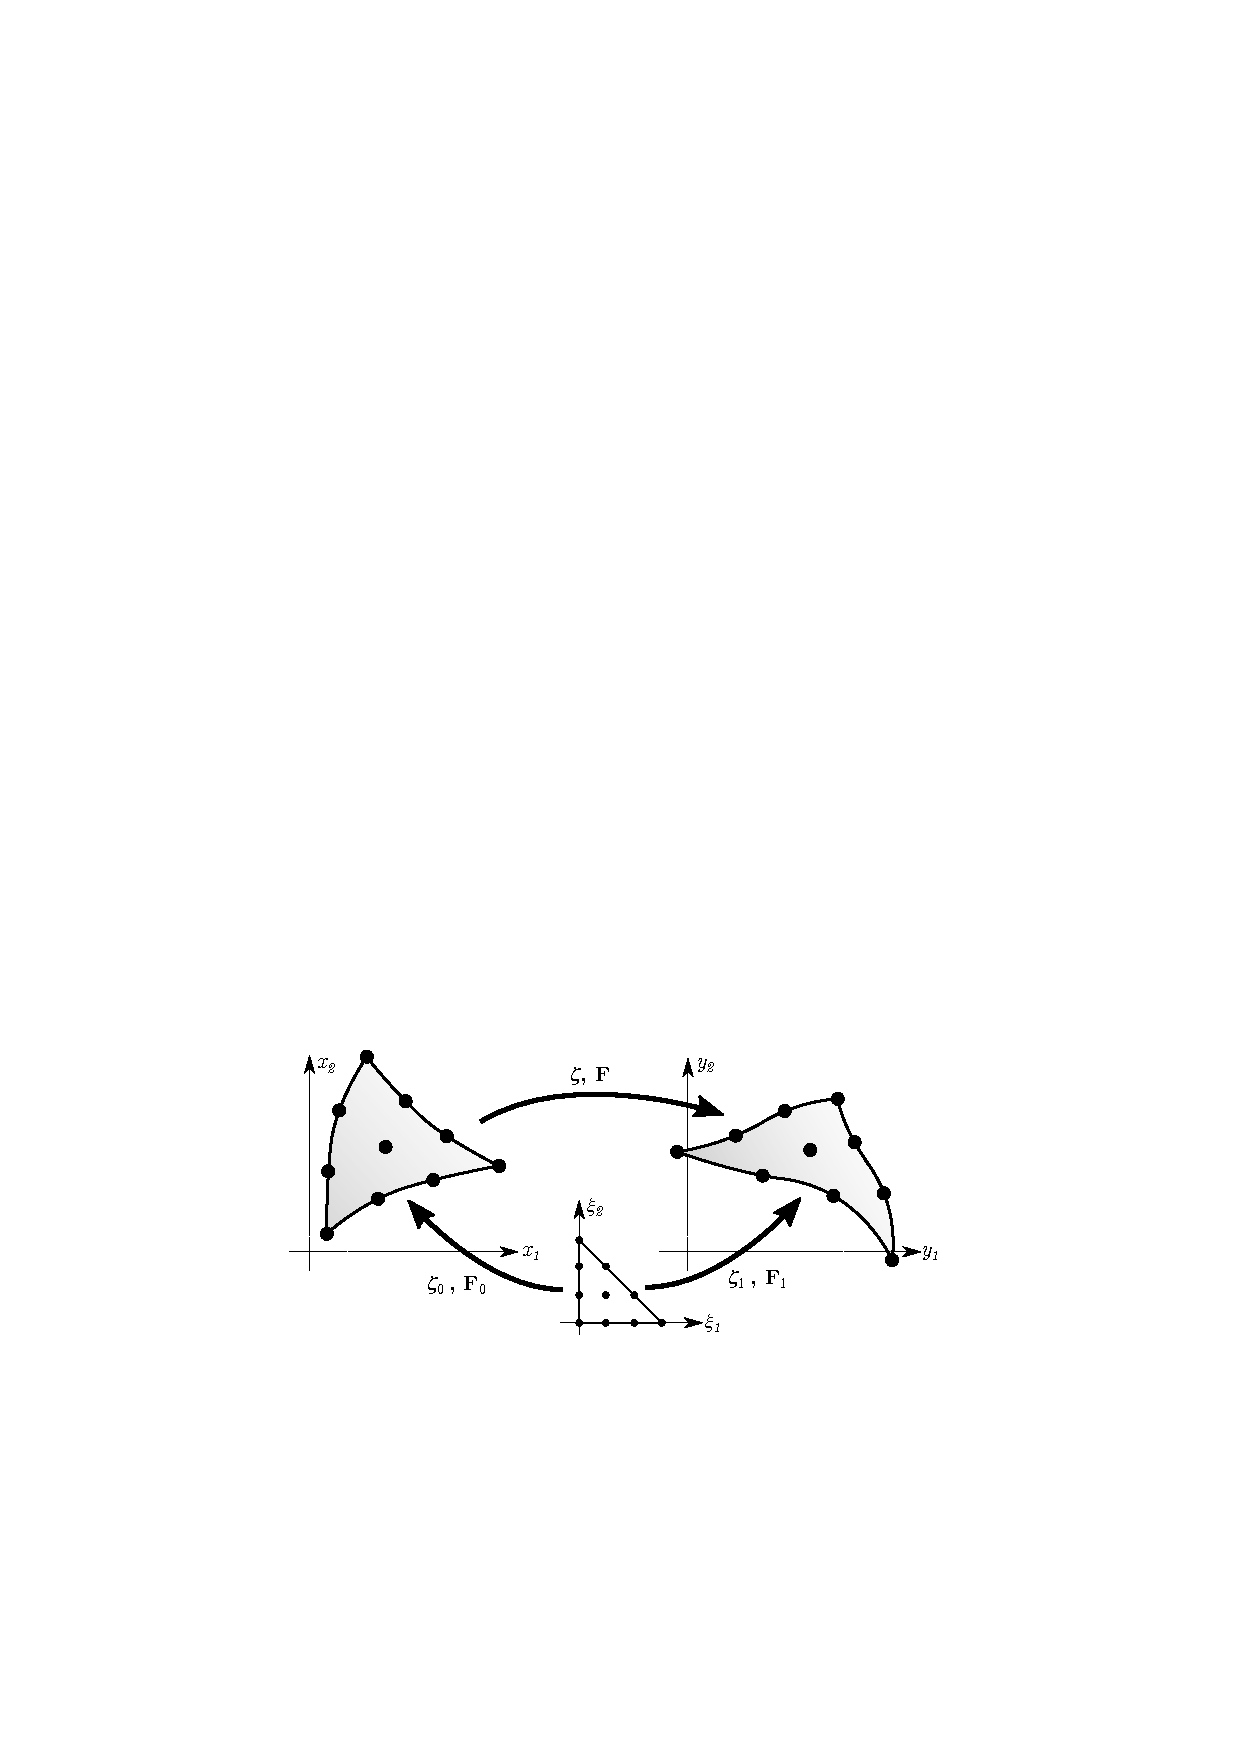
\includegraphics[scale=1.1]{Figuras/mefp.pdf}}	
	\caption*{\textbf{Fonte:} \citeonline{Pericles2019}}
\end{figure}

A partir da \cref{eq:F-FEM}, também pode se escrever a taxa do gradiente da função mudança de configuração como
\begin{equation}\label{eq:dotF-FEM}
\dotF = \dotFfin\Fini^{-1},
\end{equation}
onde
\begin{equation}
\dotFfin = \dfrac{\partial\dotfuncaof}{\partial\coords_{\;}} = \doty\nodeind\otimes\dfrac{\partial\fforma\nodeind}{\partial\coords_{\;}}. \label{eq:dotF1}
\end{equation}

Aplicando as \cref{eq:F-FEM,eq:dotF-FEM} nas \cref{eq:E,eq:dotE}, pode-se calcular o tensor de deformação de Green-Lagrange e sua taxa por meio das expressões
\begin{align}
&\E = \dfrac{1}{2}\left(\Fini^{-T}\Ffin^T\Ffin\Fini^{-1}-\I\right), \text{\,e} \label{eq:E-FEM}\\
&\dotE = \dfrac{1}{2}\Fini^{-T}\left(\dotFfin^T\Ffin+\Ffin^T\dotFfin\right)\Fini^{-1} = \text{sim}\left(\Fini^{-T}\dotFfin^T\Ffin\Fini^{-1}\right), \label{eq:dotE-FEM}
\end{align}
onde $\text{sim}(\mathbf{T}) = \frac{1}{2}\left(\mathbf{T}+\mathbf{T}^T\right)$ denota o tensor simétrico.

\subsection{Equações de equilíbrio}

Tendo escrito a equação de equilíbrio em termos do campo de posições ($\y$) e de suas derivadas temporais na \autoref{sec:equilibrio}, podemos agora escreve-la em termos dos parâmetros nodais $\y\nodeind$ e de suas derivadas temporais, usando a interpolação $\y=\fforma\nodeind\y\nodeind$. Ainda, pelo método de Galerkin, podemos tomar $\delta\y = \fforma\nodeind\delta\y\nodeind$, onde $\delta\y\nodeind$ são os valores nodais das funções ponderadoras. Assim, a variação da energia cinética, \cref{eq:dpicin}, pode ser escrita como:
\begin{equation}\label{eq:dPicin-mef}
\delta\Energiacin = \int_{\domVoli}\massi\fforma\nodeind\fforma\nodeindDois\ddoty\nodeindDois\cdot\delta\y\nodeind\,d\voli .
\end{equation}
Para as parcelas de forças externas, considerando que apenas carregamentos constantes por elemento são aplicados, temos
\begin{equation}\label{eq:dPiext-mef}
\delta\Energiaext = \int_{\domCon}\fforma\nodeind\forcaContorno\cdot\delta\y\nodeind\,d\coni + \int_{\domVoli}\fforma\nodeind\forcaVolume\cdot\delta\y\nodeind\,d\voli .
\end{equation}
Já a variação da energia de deformação pode ser reescrita como
\begin{equation}\label{eq:dPidef-mef}
\delta\Energiadef = \int_{\domVoli}\left(\S:\dfrac{\partial\E_{\;}}{\partial\y\nodeind}\right)\cdot\delta\y\nodeind\,d\voli.
\end{equation}
As integrais são calculadas neste trabalho por integração numérica, sendo realizadas no caso das \cref{eq:dPiext-mef,eq:dPidef-mef} sobre todos os elementos que contêm o nó $\node$, e no caso da equação \cref{eq:dPicin-mef} sobre todos os elementos que contêm os nós $\node$ e $\nodeDois$. Aplicando essas expressões na \cref{eq:conservacao-energia}, temos
\begin{equation}\label{eq:equilibrio-mef-0}
\left(\finer\nodeind + \fint\nodeind - \fext\nodeind \right)\cdot \delta\y\nodeind = 0,
\end{equation}
onde $\finer\nodeind$, $\fint\nodeind$ e $\fext\nodeind$ denotam, respectivamente, as forças nodais equivalentes inerciais, internas e externas do nó $\node$, cujas expressões são dadas por:
\begin{align}
&\finer\nodeind = \int_{\domVoli}\massi\fforma\nodeind\fforma\nodeindDois\ddoty\nodeindDois\,d\voli ,\label{eq:finer}\\[0.1cm]
&\fint\nodeind = \int_{\domVoli}\S:\dfrac{\partial\E_{\;}}{\partial\y\nodeind}\,d\voli ,\text{\quad e}\label{eq:fint}\\[0.1cm]
&\fext\nodeind = \int_{\domCon}\fforma\nodeind\forcaContorno\,d\coni + \int_{\domVoli}\fforma\nodeind\forcaVolume\,d\voli,\label{eq:fext}
\end{align}
Pela arbitrariedade de $\delta\y\nodeind$, a \cref{eq:equilibrio-mef-0} implica que, para cada nó $\node$, devemos ter:
\begin{equation}\label{eq:equilibrio-mef}
\residuo\nodeind = \finer\nodeind + \fint\nodeind - \fext\nodeind = \mathbf{0},
\end{equation}
isto é, o sistema global a ser resolvido consiste de $N$ equações de equilíbrio e $N$ parâmetros nodais, onde $N$ é o número de nós da discretização. Esse sistema é não-linear, sendo resolvido de forma iterativa pelo método de Newton-Raphson, cujas equação linearizadas são discutidas posteriormente na \autoref{subsec:linearizaca}.

%Sabendo que $\y = \fforma\nodeind\y\nodeind$, podemos escrever também $\doty = \fforma\nodeind\doty\nodeind$ e $\ddoty = \fforma\nodeind\ddoty\nodeind$, onde $\doty\nodeind$ e $\ddoty\nodeind$ são os valores nodais de velocidade e aceleração. Além disso, a

\subsection{Integração temporal  - Método de Newmark-$\beta$}

O método de Newmark-$\beta$ \cite{newmark1959method} é um método de integração temporal amplamente utilizado em problemas de dinâmica das estruturas. A partir dele, pode-se escrever as velocidades e acelerações em termos das posições no passo atual e no passo anterior. Parte-se das seguintes aproximações:
\begin{align}
&\y = \ys + \dotys\Delta t + \left[\left(1-2\betanewmark\right)\ddotys + 2\betanewmark\ddoty\right] \dfrac{\Delta t^2}{2}, \text{\;e} \label{eq:newmark1}\\
&\doty = \dotys + (1-\gammanewmark)\Delta t\ddotys +\gammanewmark\Delta t \ddoty, \label{eq:newmark2}
\end{align}
onde o subscrito $\notacaos$ denota que a variável é tomada no passo anterior, $\Delta t$ é o intervalo de tempo entre os passos, e as constantes $\betanewmark$ e $\gammanewmark$ são denominadas parâmetros de Newmark. Rearranjando as \cref{eq:newmark1,eq:newmark2}, é possível escrever as velocidades e acelerações no passo atual como
\begin{align}
&\doty = \dfrac{\gammanewmark}{\betanewmark\Delta t}\y + \rs - \gammanewmark\Delta t\qs \text{\quad e}  \label{eq:vel}\\
&\ddoty = \dfrac{1}{\betanewmark\Delta t^2}\y - \qs\;,\label{eq:acel}
\end{align}
onde $\rs$ e $\qs$ são grandezas que dependem apenas das variáveis no passo anterior, definidas como:
\begin{align}
&\rs = \dotys+\Delta t(1-\gammanewmark)\ddotys\text{\quad e} \label{eq:rs}\\
&\qs = \dfrac{1}{\betanewmark\Delta t^2}\ys + \dfrac{1}{\betanewmark\Delta t}\dotys + \left(\dfrac{1}{2\betanewmark}-1\right)\ddotys.  \label{eq:qs} 
\end{align}
Substituindo-se a \cref{eq:acel} na \cref{eq:finer}, as forças inerciais podem ser escritas como
\begin{equation}
\finer\nodeind = \dfrac{1}{\betanewmark\Delta t^2}\int_{\domVoli}\massi\fforma\nodeind\fforma\nodeindDois\y\nodeindDois\,d\voli - \int_{\domVoli}\massi\fforma\nodeind\fforma\nodeindDois\qs\nodeindDois\,d\voli .\label{eq:finer2}
\end{equation}

A escolha dos parâmetros de Newmark irá determinar o tipo de integração e a ordem de convergência do método. Os valores mais comumente adotados são $\betanewmark=1/4$ e $\gammanewmark=1/2$, que resultam em um integrador incondicionalmente estável de segunda ordem, e produzem resultados satisfatórios para grande parte das aplicações. Esses parâmetros, no entanto, podem provocar instabilidade numérica caso ocorram mudanças bruscas de aceleração, mobilizando frequências mais elevadas, como em problemas de impacto. Nesses casos, uma alternativa é utilizar integradores que apresentem dissipação nas altas frequências, como o de \citeonline{Hu1997}, onde adotam-se os parâmetros $\betanewmark=1$ e $\gammanewmark=3/2$.

\subsection{Linearização das equações de equilíbrio}\label{subsec:linearizaca}

A linearização das equações de equilíbrio neste trabalho é feita pelo método de Newton-Raphson, isto é, calcula-se a matriz de rigidez tangente do problema derivando a \cref{eq:equilibrio-mef} com relação aos parâmetros nodais. 

Como as forças externas são consideradas não conservativas, suas derivadas com relação às posições são nulas. Já as derivadas das forças inerciais são calculadas a partir da \cref{eq:finer2} como:
\begin{equation}
\dfrac{\partial \finer\nodeind}{\partial \y\nodeindDois_{\;\;\;}} = \dfrac{1}{\betanewmark\Delta t^2}\int_{\domVoli}\massi\fforma\nodeind\fforma\nodeindDois\,d\voli,
\end{equation}
e as derivadas das forças internas são calculadas a partir da \cref{eq:fint} como:
\begin{equation}\label{eq:fint-lin}
\dfrac{\partial \fint\nodeind}{\partial \y\nodeindDois_{\;\;\;}} = \int_{\domVoli}\left(\S:\dfrac{\partial^2\E_{\;}}{\partial\y\nodeind\otimes\y\nodeindDois} + \CC:\dfrac{\partial\E_{\;}}{\partial\y\nodeindDois}:\dfrac{\partial\E_{\;}}{\partial\y\nodeind}\right)\,d\voli
\end{equation}
onde
\begin{equation}\label{eq:CC}
\CC = \dfrac{d\S}{d\E} = \dfrac{d}{d\E}\left(\dfrac{\partial\helmholtz}{\partial\E}\right)
\end{equation}
é o operador tangente consistente do modelo constitutivo, já definido para os modelos da \autoref{sec:hiper}. As derivadas da deformação de Green-Lagrange com relação às posições podem ser calculadas pelas seguintes equações:
\begin{align}\label{eq:dE-dy}
&\dfrac{\partial\E_{\;}}{\partial\y\nodeind} = \dfrac{1}{2}\Fini^{-T}\left(\dfrac{\partial\Ffin^{T}}{\partial\y\nodeind}\Ffin + \Ffin^{T}\dfrac{\partial\Ffin}{\partial\y\nodeind}\right)\Fini^{-1} = \text{sym}\left(\Fini^{-T}\dfrac{\partial\Ffin^{T}}{\partial\y\nodeind}\Ffin\Fini^{-1}\right), \text{\quad e} \\
&\dfrac{\partial^2\E_{\;}}{\partial\y\nodeind\otimes\y\nodeindDois} = \dfrac{1}{2}\Fini^{-T}\left(\dfrac{\partial\Ffin^{T}}{\partial\y\nodeind}\dfrac{\partial\Ffin}{\partial\y\nodeindDois} + \dfrac{\partial\Ffin^T}{\partial\y\nodeind}\dfrac{\partial\Ffin}{\partial\y\nodeind}\right)\Fini^{-1},
\end{align}
onde, a partir da \cref{eq:F1}, segue que
\begin{equation}\label{eq:dF1-dy}
\dfrac{\partial\Ffinind_{ij}}{\partial\yind\nodeind_{k}} = \Iind_{ik} \dfrac{\partial\fforma\nodeind}{\partial\coordsind_{j}}.
\end{equation}



\end{document}
	
	
